\section{Einleitung}


\href{https://golatex.de/wiki/Kategorie:Befehlsreferenz}{hier geht es zur \LaTeX\ Befehlsreferenz}

\section{Umgang mit Anführungszeichen}
Das Setzen beziehungsweise die Verwendung der Anführungszeichen kann am Anfang mit \LaTeX\ ein kleines Problem darstellen.\\
\noindent
«Schweiz» 	\frqq Schweiz\flqq \\
„Deutschland“ und »Deutschland«	  	\glqq Deutschland\grqq{} und \flqq Deutschland\frqq \\
»Österreich« 	\flqq {\"O}sterreich\frqq
%« Frankreich » 	\og Frankreich\fg

\section{Umgang mit Bildern}
Bilder müssen ausserhalb von Tex abgespeichert sein und werden per Referenz eingefügt.

\noindent
\begin{minipage}{1.0\textwidth}
 	\centering
 	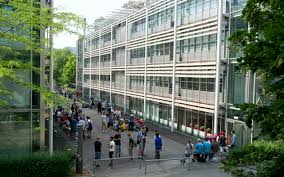
\includegraphics[width=1.0\textwidth]{Kapitel/Bilder/gibbBmSchulhausMitSchuelern}
 	\captionof{figure}{Kein Bild ohne Beschriftung!}
\end{minipage}

Um Bilder nebeneinander zu positionieren hat sich für mich folgendes Vorgehen bewährt. zuerst wird an der Stelle an welcher die Bilder eingefügt werden sollen die Verfügbare Breite "`gemessen"'.

\makeatletter
%http://groups.google.com/group/comp.text.tex/msg/7e812e5d6e67fcc5
\def\convertto#1#2{\strip@pt\dimexpr #2*65536/\number\dimexpr 1#1}	
\makeatother

\noindent
ein DIN A4 hat die Dimensionen 210 mm x 297 mm\\
an dieser Stelle ist die verfügbare Textbreite \convertto{mm}{\the\linewidth} mm

Danach kopiere ich folgender \LaTeX Code und ersetze die Breite der Bilder (hier auf 60 mm gesetzt). Ich achte darauf, dass beide Bilder zusammen nicht mehr als die angegebene Textbreite - 10mm haben. dadurch ergibt sich ein ungefährer Bildabstand von eben diesen 10 mm.

\noindent
\begin{minipage}{0.45\linewidth}
	\centering
	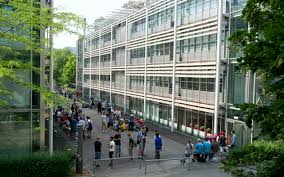
\includegraphics[width=60mm]{Kapitel/Bilder/gibbBmSchulhausMitSchuelern}
	\captionof{figure}{Start zu einer neu zu erstellenden Frage}
	\label{fig:Testbild1}
\end{minipage}\hfill
\begin{minipage}{0.45\linewidth}
	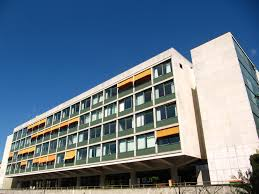
\includegraphics[width=60mm]{Kapitel/Bilder/gibbHauptgebaude.png}
	\captionof{figure}{Da sollte für jeden Geschmack etwas dabei sein}
	\label{fig:Testbild2}	
\end{minipage}

\section{Umgang mit Code}

\lstset{language=TEX}
Code wir in der speziellen Umgebung \lstinline$\lstlisting$ gesetzt, zum Beispiel: Java \lstset{language=Java} \lstinline$boolean b=true;$ oder Python \lstset{language=Python} \lstinline$sum = float(num1) + float(num2)$ 

mehre Zeilen:
\begin{lstlisting}
if(<boolescher Ausdruck>){
// Anweisung(en)
} else {
// Anweisung(en)
// Anweisung(en)
}
\end{lstlisting}

\section{Ausstehende Arbeiten} \label{sec:AusstehendeArbeiten}

\begin{itemize}
	\item Titelfonds
	\item das Layout für die \glqq Normalen\grqq{} Seiten
	\item Alle diese komischen Boxen :-)
	\item Alle Fonts setzen (auch wenn die vorgestellten wehtun...)
\end{itemize}

\blindtext[5]

